\documentclass[10pt]{article}
%\usepackage{epsf}
%\usepackage{graphics}
%\usepackage{fullpage}
\usepackage{graphicx}
\usepackage{multirow}
\usepackage{makeidx}
\usepackage{latexsym}
\usepackage{bm}
\usepackage{amsmath}
\usepackage{amsthm}
\usepackage{amssymb}
\usepackage{setspace}
\usepackage{natbib}
 
\onehalfspacing
%\doublespacing
\setlength{\textheight}{22.5cm}
\setlength{\textwidth}{6.47in}
\setlength{\oddsidemargin}{-1mm}
\setlength{\topmargin}{0.1cm}
\setlength{\evensidemargin}{-5mm}
\makeindex

\newcommand{\captionfonts}{\footnotesize}
\makeatletter  
\long\def\@makecaption#1#2{
  \vskip\abovecaptionskip
  \sbox\@tempboxa{{\captionfonts #1: #2}}
  \ifdim \wd\@tempboxa >\hsize
    {\captionfonts #1: #2\par}
  \else
    \hbox to\hsize{\hfil\box\@tempboxa\hfil}
  \fi
  \vskip\belowcaptionskip}
\makeatother

\newcommand{\ts}{^{\sf T}} 
\newcommand{\its}{^{\sf -T}}

\begin{document}
\title{within area distance paper...}

\author{David L. Miller and Simon N. Wood,
\\ Mathematical Sciences, University of Bath
}


\maketitle
\begin{abstract}
Here we investigate the utility of within-area distance based smoothing techniques for generalised additive models.


%\vspace{0.4cm}
%\noindent \textbf{Keywords:} 
\end{abstract}

\section{Finite area smoothing}

Splines are a popular way of performing spatial smoothing in two dimensions. In this context, they are often used to fit smooth functions over a geographical region. A typical application of this is in ecological modelling; a response (for example the presence of individuals in a population or concentration of a chemical) is modelled as a function of its spatial coordinates. The estimated function can then be used to perform inference on the population, whether that be an abundance estimate, density map or a more sophisticated inferential goal. Finite area smoothing simply specifies that the domain over which this smoothing takes place is bounded.

When the geographical region has a \emph{complex boundary}, features from one part of the domain can unduly influence other parts. Considering the boundary as a polygon, a complex boundary is a non-convex polygon, in particular when the non-convexity is relatively extreme. Often this consists of having some peninsula-like feature(s) in the domain with notably different observation values on either side of the feature. Given that there is some scientific motivation as to why those parts of the domain should not affect each other, features such as peninsulae give rise to a phenomenon known as \emph{leakage}.

Leakage occurs when a smoother inappropriately links two pats of a domain (\cite{soap}). The phenomenon is problematic since it causes the fitted surface to be mis-estimated; this can then lead to incorrect inference (e.g. biased abundance estimates), which is clearly not desirable. Leakage can be seen in figure \ref{leakage} where the high values in the upper half of the domain leak across the gap to the lower values below and vice versa.

% leakage example 
\begin{figure}
\centering
% trim order l b r t
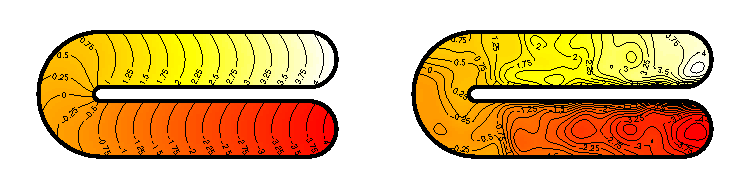
\includegraphics{figs/ramsay-leak.pdf}\\
\caption{An example of leakage. A thin plate regression spline was fit to data sampled from the function on the left, here the model smooths across the gap in the middle of the domain (right.)}
\label{leakage}
\end{figure}

The problem of leakage arises because of the way in which the smoother defines how near objects are to one another. Most smoothing techniques use the Euclidean metric to measure the distance between data. Clearly though, this approach is a flawed: biological populations do not conform to Euclidean geometry in their movement patterns and hence their observed positions will reflect this. Just as whales no not uniformly distribute themselves across sea and glacier, fish do not lay their eggs on land. Natural and man-made barriers carve up the landscape (and seascape), partitioning biological populations; our models should take this into account.

The distribution of the population may be smooth, just not necessarily over $\mathbb{R}^2$ (\cite{wangranalli}). Instead the structure of the domain that is under investigation must be modelled (implicitly or explicitly) for the correct inference to be drawn.

\subsection{Ramsay's horseshoe function as a benchmark for finite area smoothing}

\label{ramsayfunc}

\cite{ramsay} proposes a function which can be used to benchmark new approaches to 2-dimensional smoothing. The function takes the form of a horseshoe shape which is flat across the domain has a gradient along the domain's major axis. This can be seen in figure \ref{orig-fs}. \cite{soap} modify the test function by adding curvature across the minor axis of the shape. This was added in order to avoid the horseshoe function lying in the nullspace of their model's penalty, making the problem trivial. It is the second shape that will be used for simulations here and shall be referred to as the \emph{Ramsay horseshoe} throughout; it is shown in figure \ref{leakage}.

% original horseshoe from Ramsay's paper
\begin{figure}
\centering
% trim order l b r t
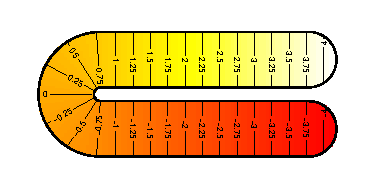
\includegraphics{figs/orig-fs.pdf}\\
\caption{The horseshoe function as it appeared in \cite{ramsay}.}
\label{orig-fs}
\end{figure}

The test function highlights the problem of leakage very well. As mentioned above, when the smoothing problem is specified in terms of Euclidean distance, the model takes the distance between the points in the two arms of the horseshoe as the distance over the gap in-between them, rather than the distance along the major axis of the shape. This causes the high function values from one side to contaminate the other side (and the low to contaminate the high.) It is easy to see that this causes the smooth to be an inappropriate model.

\subsection{Previous approaches}

The cause of leakage can be characterised in two ways: either the smooth does not respect the boundary of the domain, or the smooth does not take into account the geometry of the domain (in particular with regard to the distance between points within the domain). Previous work in this area has been to combat leakage along these two lines. 

%Work of \cite{ramsay} and \cite{soap} both use a partial differential equation (PDE) boundary condition approach to try to prevent leakage, where as \cite{wangranalli} and \cite{eilerstalk}  attempt to approximate the intrinsic structure of the domain while not treating the boundary as something special in the basis setup. These four main works may be summarised as follows:

\begin{itemize}
\item \cite{ramsay} proposes finite element $L$-splines (FELSPLINEs). The procedure begins by triangulating the domain. For each triangle a set of bivariate quadratic polynomial basis functions are constructed, with continuity specified over their edges. These functions are used to form the spline which has the  penalty:
\begin{equation}
\int_\Omega (L_p f)^2 \text{d}\Omega,
\end{equation}
where $\Omega$ is the domain in question and $L_p$ is a roughness operator defined as:
\begin{equation}
L_p=\Delta^p+c_{p-1}\Delta^{p-1}+\dots+c_1\Delta+c_0I.
\end{equation}
Here $I$ is the identity operator, the $\{c_0,\dots, c_p\}$ are constants and the $\Delta$ is the Laplacian ($\Delta f = f_{xx}+f_{yy}$ in the usual notation). Although any differential operator could, in principle, be used for $L_p$, the Laplacian gives rise to a set of polynomials which are rotation and translation invariant which ensures that the solution is coordinate system invariant.

Since the triangulation and hence the penalty of the FELSPLINE is only calculated over the domain, and the continuity is specified over neighbouring cells, the method prevents leakage. However, although FELSPLINE does not exhibit leakage on the original horseshoe (as in figure \ref{orig-fs}), in practice the model makes unrealistic physical assumptions. The boundary conditions of FELSPLINE specify that the gradient is zero, along normals to the boundary. This is not always physically realistic. \cite{soap} show that by using a different response function for the horseshoe shape, the FELSPLINE performance begins to falter.

FELSPLINE does not offer a realistic physical model and is therefore not a viable solution to the finite area smoothing problem in general.

\item \cite{wangranalli} adopt a ``within-area distance'' formulation for thin plate splines. They choose to use the geodesic distance between two points, that being the shortest path within the domain. This gives a definition of how near objects are in the domain. This is then used as the distance in the radial basis functions of a thin plate spline, rather than using the usual Euclidean distance, they refer to this as GLTPS.

Wang and Ranalli first create a weighted, undirected graph ($G$, say) with a data point at each vertex and the distance between each pair of vertices as the weights on the edges. They then take the restricted graph of $G$, $G_k$, in which each vertex is only connected to its $k$ nearest neighbours. With this new, restricted graph the geodesic distances between each pair of vertices can be calculated using Floyd's algorithm (\cite{Floyd}).

As the authors point out, the quality of the approximation is dependent on the size of the data set and its density. At low densities the estimated geodesic distance will tend towards the Euclidean, at high densities the approximation tends, asymptotically toward the true geodesic distance (\cite{bernstein}). Even if  dense enough data were available, the method will be rather slow since Floyd's algorithm is cubic in the number of vertices (the size of the data set). Finally, although the $k$-nearest neighbours algorithm used is not specified in the paper, in general such procedures are computationally expensive, adding another source of impedance to the technique.

\textbf{Write about the penalty problem here.}
Since the method only uses the geodesic distances in the radial basis functions of the thin plate spline (see, for example \cite{simonbook},  p. 154) but not the unpenalised (those residing in the nullspace of the usual penalty), a knot-based approach must be used with a ridge-type penalty rather than the approach of \cite{wood2003}. This is because if the latter approach is taken, the square root of the smoother matrix cannot be taken (since there are negative eigenvalues).


Taking these points into account, Wang and Ranalli's approach appears cumbersome, slow and dependent on dense data.

\item The soap film smoother (\cite{soap}) uses a rather simple physical model to prevent leakage from occurring. First, consider the domain boundary to be made of wire, then dip this wire into a bucket of soapy water, you will then have (provided it doesn't pop(!)) a soap film in the shape of your boundary. Now consider the wire to lie in the $x-y$ plane and the height of the soap film at a given point to be the functional value of the model. This film is then distorted smoothly by moving it toward the data, while minimising the surface tension in the film. The domain ($\Omega$) is bounded by some polygon with boundary conditions that are either known or estimated by a cyclic spline.

\textbf{Do I need to go into this much detail?}

Mathematically, the soap film smoother is constructed by first specifying a set of functions $\rho_k(x,y)$, which are each solutions to the Laplace equation in two dimensions:
\begin{equation}
\frac{\partial^2\rho}{\partial x^2} + \frac{\partial^2\rho}{\partial y^2} = 0
\end{equation}
except at one of the knots ($x^*_k,y^*_k$). Then, solving Poisson's equation in 2-dimensions:
\begin{equation}
\frac{\partial^2 g_k}{\partial x^2} + \frac{\partial^2 g_k}{\partial y^2} = \rho
\label{soap-poisson}
\end{equation}
with $\rho=\rho_k(x,y)$, where $k$ indexes the knots and the boundary condition $\rho=0$. The set of basis functions for the soap film smoother, $g_k(x,y)$ is found, along with $a(x,y)$ (the solutions to (\ref{soap-poisson}) when $\rho=0$, subject to the boundary condition). These bases are then summed to form:
\begin{equation}
f(x,y)=a(x,y)+\sum_{k=1}^n \gamma_k g_k(x,y),
\end{equation}
the soap film smoother, where the $\gamma_k$ are parameters to be estimated. The (isotropic) penalty term (GAMpenalties) is:
\begin{equation}
\int_\Omega \Big(\frac{\partial^2 f}{\partial x^2}+\frac{\partial^2 f}{\partial y^2} \Big)^2\text{d}x\text{d}y,
\end{equation}
Differing from the standard thin plate regression spline penalty since: (\emph{i}) the integration occurs only over $\Omega$, (\emph{ii}) there is no mixed derivative term, and (\emph{iii}) the whole integrand is squared rather than each term individually. This allows the $x$ and $y$ term's derivatives to be traded off against each other so the nullspace of the penalty is infinite dimensional. This allows those functions in the nullspace to be sufficiently wiggly to meet any boundary conditions.

The solution of the PDEs above, yielding the basis and penalty, is the most computationally expensive part of the procedure. Knots to use for $x_k^*$ and $y_k^*$ must be specified, usually using a grid. Numerical problems occur when knots are placed in boundary cells in the PDE solution grid.

Although mathematically elegant, the soap film smoother is a rather complex model. It also treats the boundary differently from the interior and uses a cyclic spline in order to approximate the boundary values. 

\textbf{Do we want to talk about soap at all?}

\item An alternative approach to treating the boundary as something special is to transform the space in which the points lie to instead lie in a different domain which is more suitable for smoothing. For example, with Ramsay's horseshoe, it seems intuitive to simply bend the horseshoe into a long strip and then smooth on that domain. Indeed, \cite{eilerstalk} proposed using the Schwarz-Christoffel transform (\cite{driscoll}) for this very purpose. 

The basic idea is to find a function, $\varphi$ say, that takes points in the domain the data lie in ($W$) and maps them to a domain ($W^*$) in which the boundary is less complex ($\varphi : W \mapsto W^*$, mathematically).

Creating some kind of mapping between the space in which the data lies and the space in which conventional smoothers perform well is convenient. Not having to setup a new basis structure is clearly appealing. This approach also benefits from not treating the boundary as a special in the basis setup.

The authors have investigated this approach further and have found it to not be generally applicable. For shapes such at the horseshoe there are obvious transformations that make the mapping straightforward. However, in more realistic examples (like, say, a coastline or river system) the domain to map to is not clear. The Schwarz-Christoffel mapping allows mapping only into a restricted set of domains (most common are the unit disk, upper half-plane and rectangle), during their investigations the authors (\textbf{should I be talking about myself in the third person?}) found that using the mapping caused a severe breakdown of isotropy, causing artefacts in the smooths produced. 

\item MDS+TP + Curriero
\end{itemize}

\section{Aim and scope of this article}

Aim here is to compare a set of WAD-based methods, what are the general problems, when can they be useful.

\section{Within area distance - why?}





\section{Our approach}

Set out the models to be compared here.




\section{Simulation experiment}

Simulation settings same as W+R paper. 200 realisations, 100 samples, noise=0.05, 40 knots selected using the \texttt{cover.design()} function in \texttt{fields}. Use a simplified boundary for speed: take every 5th vertex on the curved parts of the boundary. Predicated back over 

Compare the following models:

\begin{itemize}
	\item MDS+tprs
	\item MDS+tps
	\item soap film smoother
	\item WR+tps
\end{itemize}

Calculated MSE, 

% MSE plot
\begin{figure}
\centering
% trim order l b r t
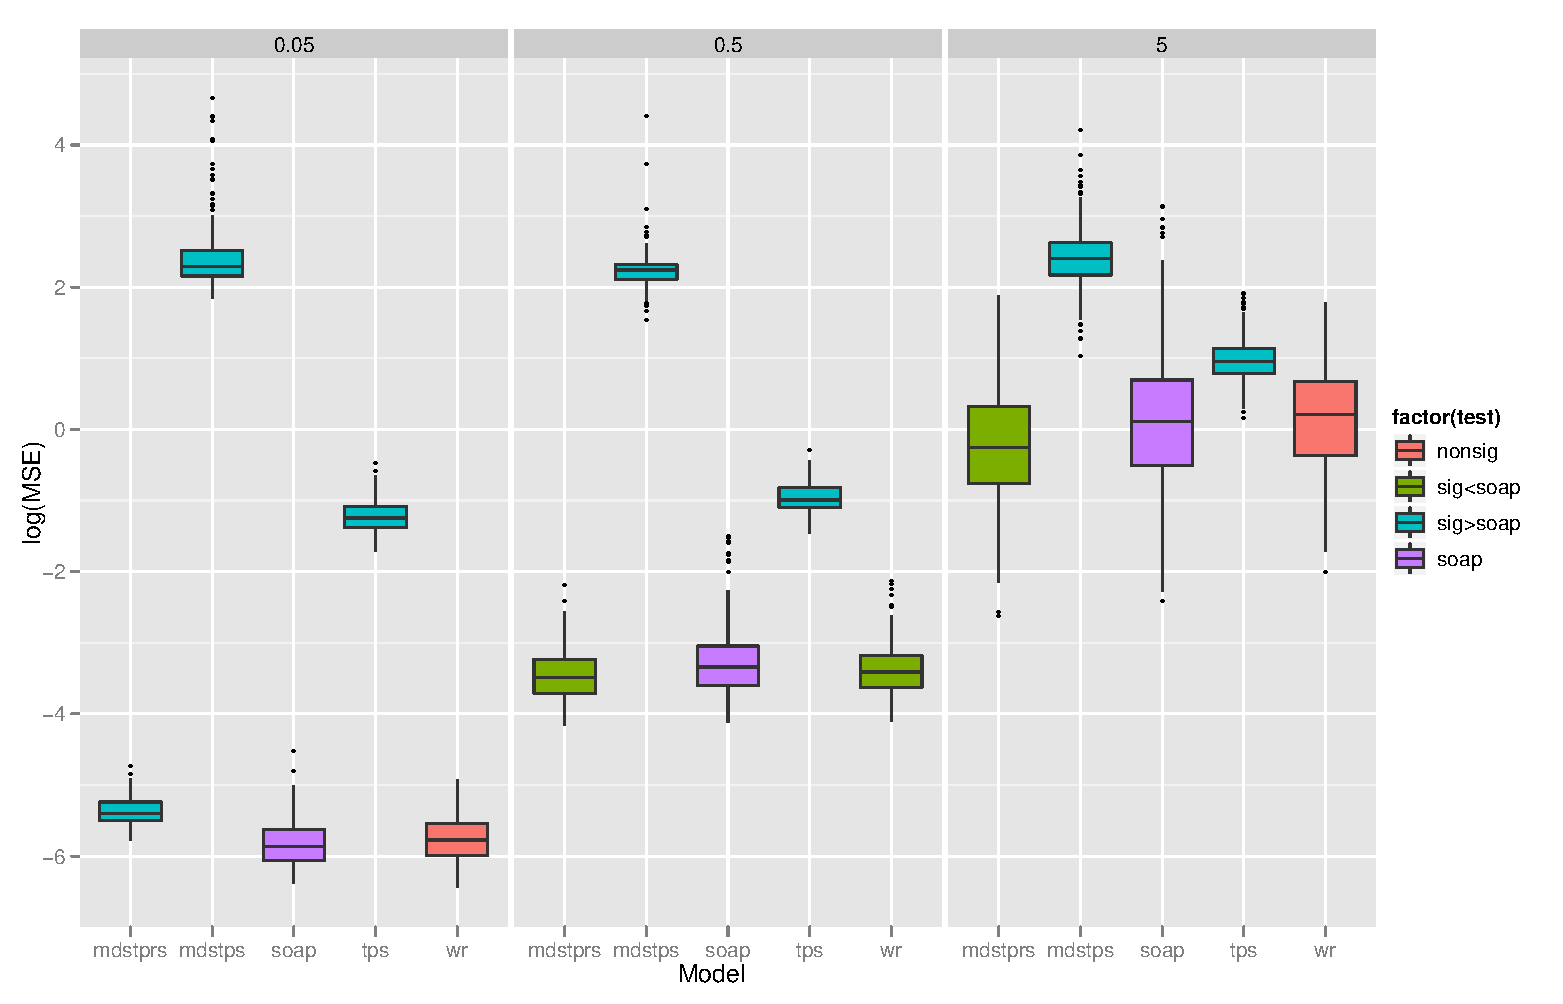
\includegraphics[width=6.5in]{figs/ramsim-mse.pdf}\\
\caption{Boxplot of MSE}
\label{ramsim-mse}
\end{figure}


0.05\\
soap vs.  tps 1.447002e-34 \\
soap vs.  wr 0.0136878 \\
soap vs.  mdstps 1.447002e-34 \\
soap vs.  mdstprs 2.508476e-26 \\

0.5\\
soap vs.  tps 1.447002e-34 \\
soap vs.  wr 0.0001010435 \\
soap vs.  mdstps 1.447002e-34 \\
soap vs.  mdstprs 1.028156e-06 \\

5\\
soap vs.  tps 1.224688e-16 \\
soap vs.  wr 0.5446379 \\
soap vs.  mdstps 4.034417e-32 \\
soap vs.  mdstprs 8.986215e-09 \\





%also ``artefactiness'':
%\begin{equation}
%\label{artedef}
%A= \int\int_\Omega  \Big( \frac{\partial^2 (f_m(x,y)-f_t(x,y))}{\partial x^2}\Big)^2 + \Big(\frac{\partial^2 (f_m(x,y)-f_t(x,y))}{\partial x \partial y}\Big)^2 + \Big(\frac{\partial^2 (f_m(x,y)-f_t(x,y))}{\partial y^2}\Big)^2 \text{d}x\text{d}y.
%\end{equation}
%where $f_m(x,y)$ is the model and  $f_t(x,y)$ is the truth. This is supposed to measure the wigglyness in the difference between the two, giving an idea of whether there are artefacts in the smooth.
%
%% artefactiness plot
%\begin{figure}
%\centering
%% trim order l b r t
%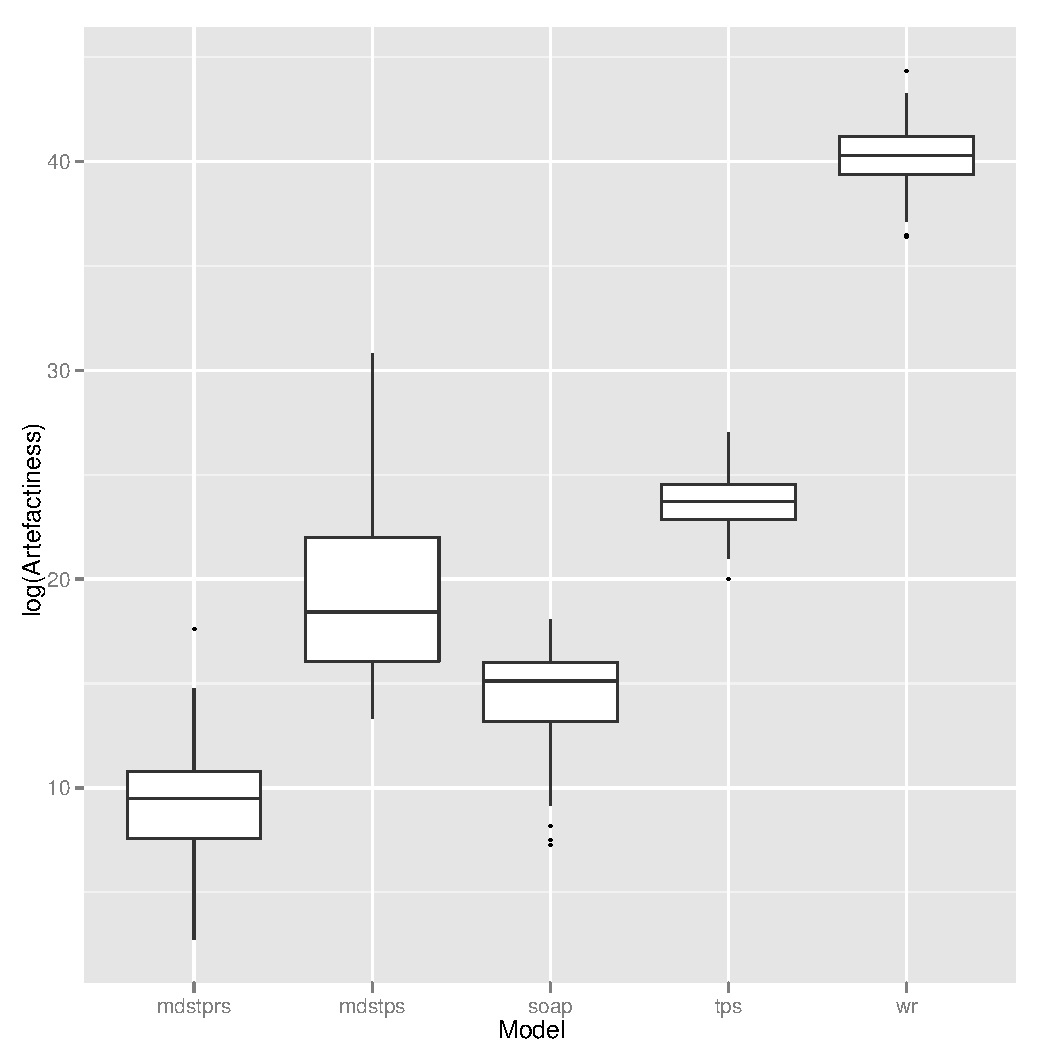
\includegraphics[width=4in]{figs/arteboxplot.pdf}\\
%\caption{Boxplot comparing the models tested for ``artefactiness'' as defined in (\ref{artedef}).}
%\label{arteboxplot}
%\end{figure}



\section{Conclusions}



\bibliographystyle{chicago}
\bibliography{bib-hell}



\end{document}



